%% ----------------------------------------------------------------------
%% apa7 - A LaTeX class for formatting documents in compliance with the
%% American Psychological Association's Publication Manual, 7th edition
%% 
%% Copyright (C) 2019 by Daniel A. Weiss <daniel.weiss.led at gmail.com>
%% 
%% This work may be distributed and/or modified under the
%% conditions of the LaTeX Project Public License (LPPL), either
%% version 1.3c of this license or (at your option) any later
%% version.  The latest version of this license is in the file:
%% 
%% http://www.latex-project.org/lppl.txt
%% 
%% Users may freely modify these files without permission, as long as the
%% copyright line and this statement are maintained intact.
%% 
%% This work is not endorsed by, affiliated with, or probably even known
%% by, the American Psychological Association.
%% 
%% ----------------------------------------------------------------------
%% 
\documentclass[man,floatsintext]{apa7}

\usepackage{graphicx}        % provides \resizebox
\usepackage{enumitem}
\usepackage{setspace}
\usepackage[american]{babel}
\usepackage{float}
    \usepackage{graphicx}
    \usepackage{capt-of}
    % \usepackage{caption}

\usepackage[font=small,skip=0pt]{caption}
\usepackage{csquotes}
\usepackage[style=apa,sortcites=true,sorting=nyt,backend=biber]{biblatex}
\DeclareLanguageMapping{american}{american-apa}
\addbibresource{bibliography.bib}

% maps apacite commands to biblatex commands
\let \citeNP \cite
\let \citeA \textcite
\let \cite \parencite

\title{Plant Pathology Image Classification}
\shorttitle{Plant Pathology Image Classification}

\author{Bi Nguyen}
\affiliation{University of California - Davis, ECS 171: Machine Learning, Professor Setareh Rafatirad, 5 December 2021}

\begin{document}
\maketitle

\begin{singlespace}
\section{Introduction}
With the world population growing exponentially, food scarcity remains a major threat in many countries. It is expected by 2050, the world population is projected to reach nearly over 10 billion people with a growing food demand between 59$\%$ and 98$\%$ \parencite{elferink}. Agricultural farming contributes to 70$\%$ to 80$\%$ of the world's food, respectively to any family farm size \parencite{ritchie}. Not only that, but these farmers rely heavily on their crops for survival. So it is important to help farmers be successful in producing healthy crops for the sake of their livelihood as well as everyone's.

One of the many issues of crop failure is plant pathogens. These diseases drive food production down and increase the cost of treatment, and manually identifying the different underlining diseases can be time-consuming and costly. Therefore, it is crucial to identify the correct disease to apply the proper chemicals that help the crops and provide nutrients to the soil \parencite{chemicals}. With the rapid emergence of smartphones with different image capturing capabilities and recent developments in computer vision, we can help farmers reduce the misuse of chemicals that negatively affects the crops and environment by using deep neural network specifically convolutional neural network for image classification.


\section{Method}
\subsection{Data Description}
The dataset contains 3,240 images with 4 labels assigned to them. Figure~\ref{fig:Figure1} shows the images of the different classes assigned to them. Most of the images came with the same resolution of 2044 x 1369 pixels while some came at the inverse resolution of 1369 x 2044. 

\begin{figure}
  \centering
  \caption{Class Labels}
  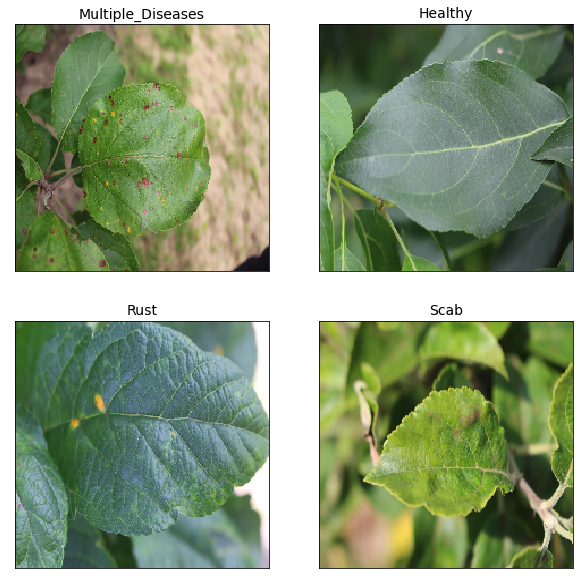
\includegraphics[width=0.45\textwidth]{images/image1.png}
  \label{fig:Figure1}
\end{figure}

In order to apply any machine learning model to these images, I had to rescale them to different sizes. During the initial trials with different resolutions, I found that 224 x 224 pixels were the optimal size because it still captures the important details of the plant leaves while being computationally feasible. Figure~\ref{fig:Figure2} shows the rescaling of the original image to 224 x 224 pixels. You can see still see the marker that identifies this leave has multiply diseases.

\begin{figure}
  \centering
  \caption{Reduce Resolution}
  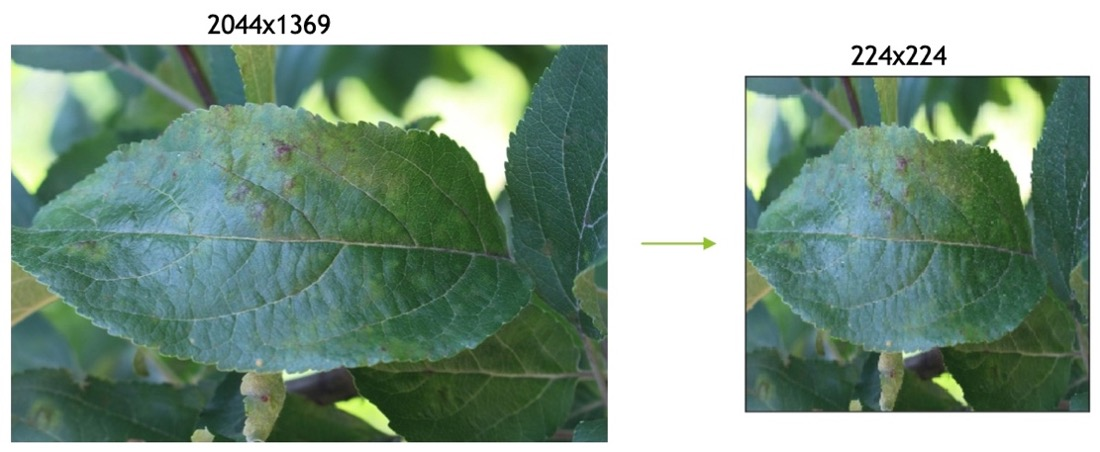
\includegraphics[width=0.75\textwidth]{images/image2.jpg}
  \label{fig:Figure2}
\end{figure}

Note that of those images, half of them are divided as training set and the other as test
set. That means only about 1,600 images are labeled and used to train the deep neural network. So how can we test the accuracy of our model performance? By splitting 20$\%$ of the training samples into a validation. Since our sample size decreased even more, this will possibly affect the performance of our model. Ideally, in any neural network, the more samples we have, the better the model will be at making predictions. Think of it this way, if we were to look at different images of different cat breeds, it is likely that we won’t remember them after only seeing a few images. Therefore, if we were to look at many pictures of the same label, then we will be better at identifying the pattern for a particular label. This same idea applies to machine learning models.

As a result of subsetting the training data, the features in the training set contains 77
images of plants with multiple diseases, 405 images of healthy plants, 511 images of plants with rust, and 463 images of plants with scab while the validation consists of 14 images of plants with multiple diseases, 111 images of healthy and rust plants and 129 images of plants with scab.
Notice that the distribution of plants with multiple diseases is smaller compared to the other 3
labels. This means that our model might not be good at classifying plants with multiple diseases
because it doesn’t nearly have enough data to recognize patterns that can describe this class label.


\subsection{Approach}
If we take a look at Figure~\ref{fig:Figure1} again, notice that there are different variations in how the
images have been taken. Each picture can have a different orientation, height, and width,
whether it’s zoomed in or not, blurry background, and level of brightness. All of these distinctions and combinations need to be addressed when building our model. We want to address this issue because due to the lack of data, accounting for different ways of how the images are taken can help generalize our model and prevent overfitting. Figure~\ref{fig:Figure3} display an image with different sets of variations. 

\begin{figure}
  \centering
  \caption{Image Augmentation}
  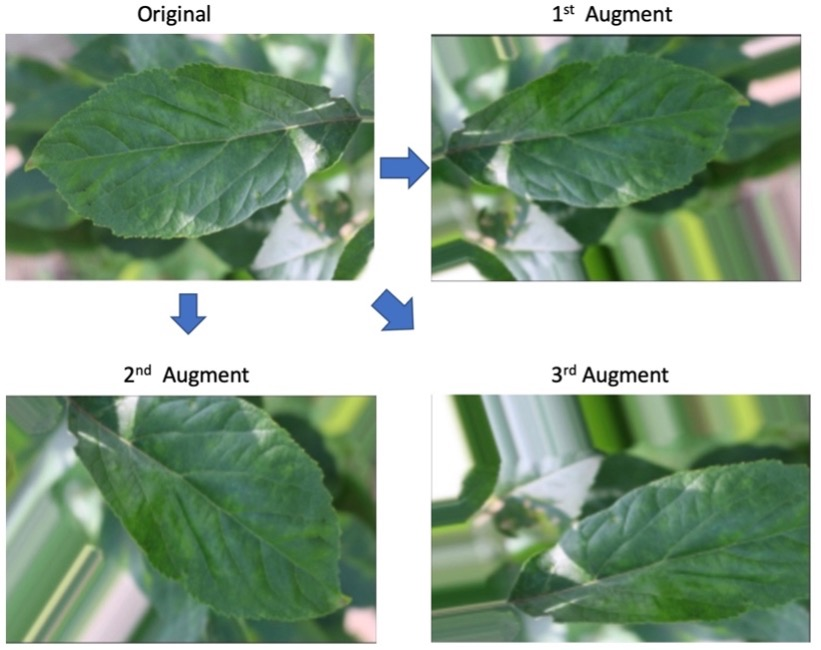
\includegraphics[width=0.5\textwidth]{images/image3.jpg}
  \label{fig:Figure3}
\end{figure}

From the above images, you can see that these transformations can add additional data
to our model so that it can generalize different images and hopefully improve the model’s
performance. Note that the images are augmented randomly with the following settings:
\begin{itemize}[itemsep=1mm, parsep=0pt]
  \item Rotation Range: 45°
  \item Brightness Range: [0.2, 0.5]
  \item Height Shift Range: 0.2
  \item Width Shift Range: 0.2
  \item Zoom Range: 0.2
  \item Horizontal Flip, and Vertical Flip
  \item Fill mode: Nearest
\end{itemize}

I choose these settings because it resembles how some of the images are taken in the dataset.

\subsection{Building the Model}
I used a Convolutional Neural Network (CNN) for image classification compared to a
Multilayer Perceptron Model (MLP) because of its ability to be efficient, account for the spatial locality, and it's translational invariant. What I mean is that, if an MLP model is given a 224 x 224 pixels input with 3 color channels then that means there are over 150,000 inputs that have to be trained. That is computationally expensive and can cause overfitting due to a large number of variables. Furthermore, MLP does not account for the different positions that an object might be in. It will assume the object's location and try to adjust its weights to place it there \parencite{stewart}. CNN on the other hand takes all these factors into account through the use of filtering and pooling.

Our model consists of 3 convolutional layers, and for each layer, there is a 3x3 filtering window and a max-pooling of size 2. These settings are chosen because of the input size of our image. If we had computational power, then we can improve the resolution to over 500 pixels and try different settings for each layer. Nevertheless, our model takes in an image that is 224 x 224 pixels scaled down to [0, 1] for ease of computation. Then it goes through the first convolutional layer where it extracts certain feature that makes up the plant leave such as the edges and corners of the image. This feature extraction is done by the filtering and max-pooling window. Essentially, the filtering layer calculates the dot product of its weight (a 3x3 matrix with randomly assigned weights) with the top-left window of the input matrix and continues to do so until the window has slid through the entire matrix. This output will then be used as input for the
max-pooling layer where it extracts the pixels that are most concentrated. Similarly for the next 2 convolutional layers, the output of the previous layer is used as input for the next until we reach the end where we have to flatten the matrix to create a 1D feature vector to connect to the fully connected layer to classify the class labels for the plants. Figure~\ref{fig:Figure4} shows how the image gets processed as it goes through the different stages of the neural network.

\begin{figure}
  \centering
  \caption{Stages of the Convolutional Layers}
  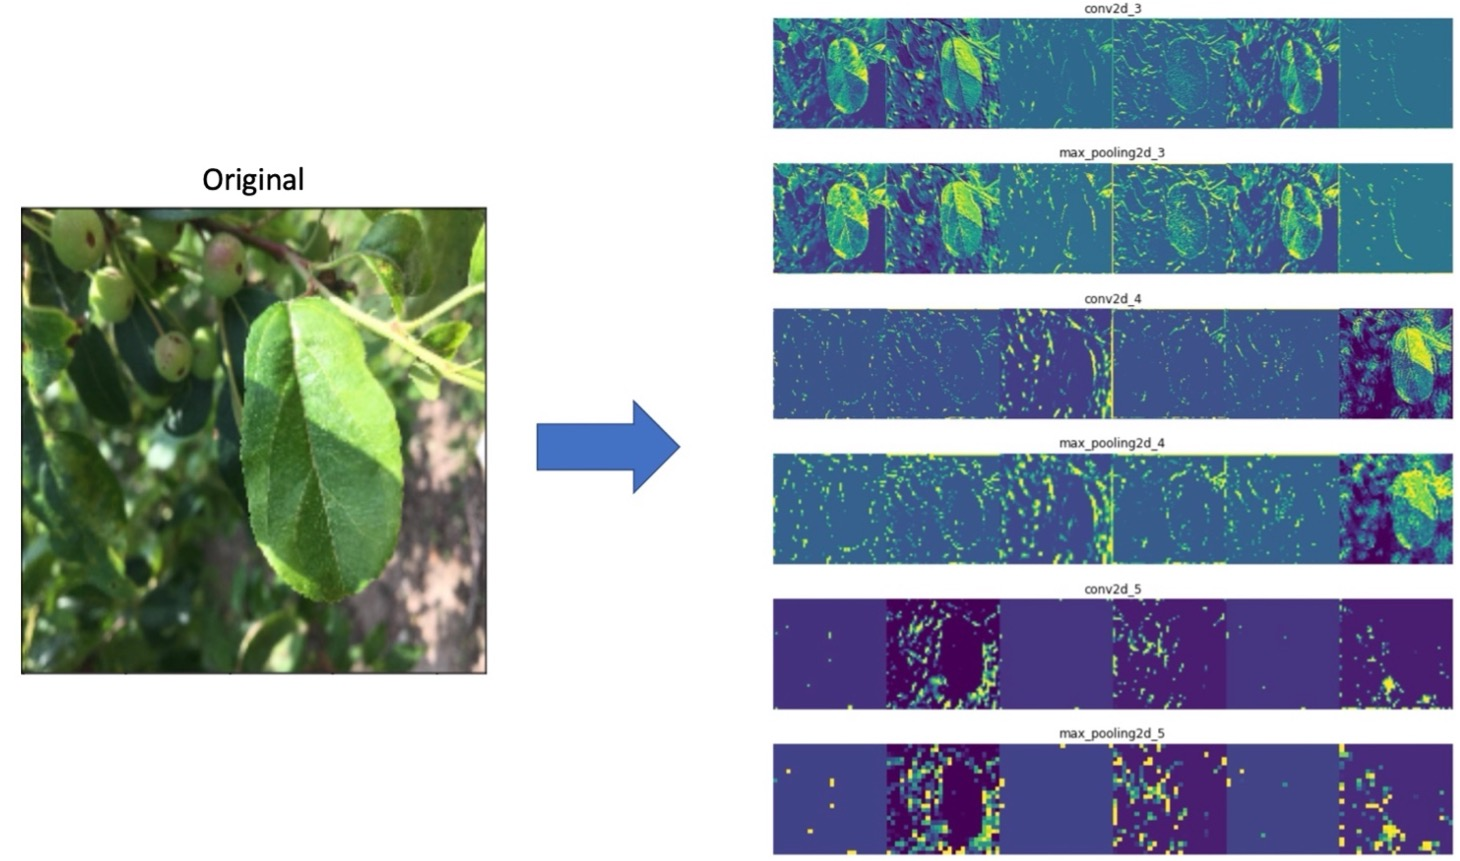
\includegraphics[width=0.8\textwidth]{images/image4.jpg}
  \label{fig:Figure4}
\end{figure}

As you can see from the image on the right, initially the first layer still keeps the details that make up the plant. But, as you go deeper into the 2nd and 3rd layers, you can see how the image is an abstraction of what it used to be. This is the model trying to perform feature extraction to determine the label for this image.

The model that build the images above consists of the following settings:
\begin{itemize}[itemsep=1mm, parsep=0pt]
  \item 30 Training Iterations (Epochs)
  \item Dropout Layer of 0.02 for regularization to avoid additional overfitting
  \item Adam optimizer with learning rate of 0.0001
  \begin{itemize}[label=$\circ$]
    \item I chose this optimizer because it already incorporate mometum as
part of gradient descent.
    \end{itemize}
  \item Relu activation for all the convolutional layers
  \item Padding on the images
  \item Accuracy as a metric of performance
  \item Batch size of 32
\end{itemize}

\subsection{Model Performance}
As a result of our data pre-processing and analysis, we obtain an 80$\%$ accuracy rate. This is relatively decent considering that we have a small-sized data set. Figure~\ref{fig:Figure5} shows the performance of the model through each epoch.

\begin{figure}
  \centering
  \caption{Model Performance}
  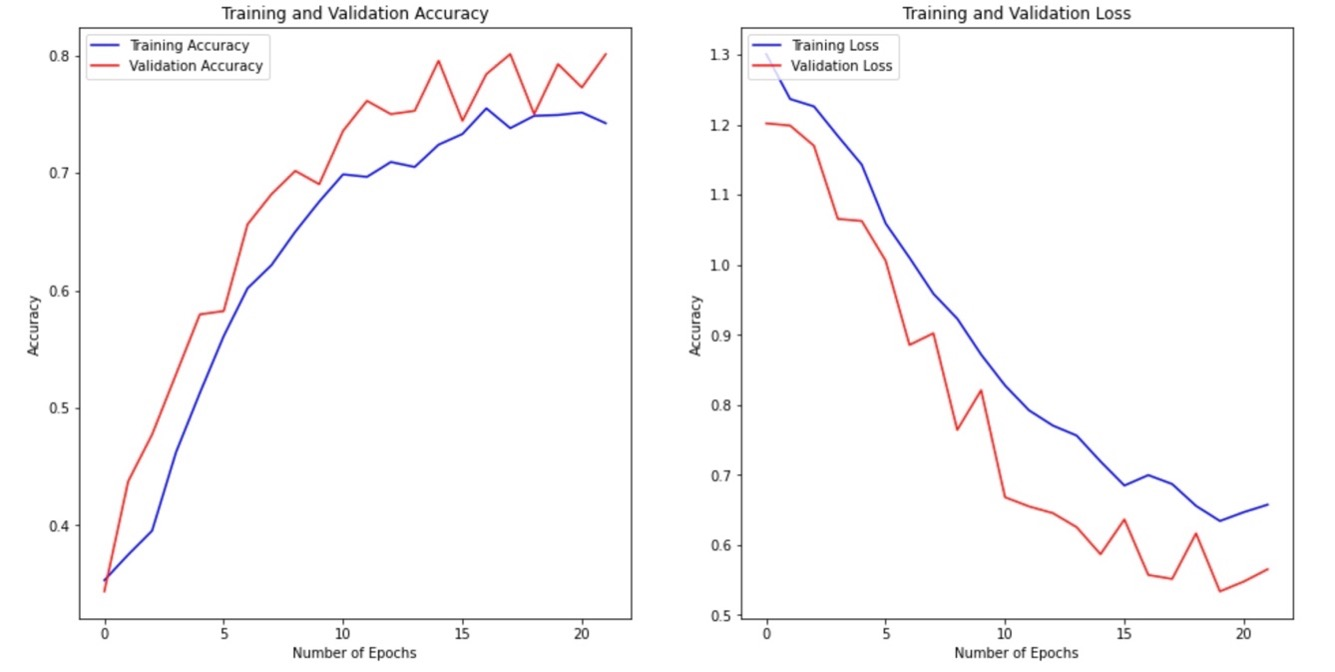
\includegraphics[width=1\textwidth]{images/image5.jpg}
  \label{fig:Figure5}
\end{figure}

As you can see from the images above, our model performs quite poorly in the initial stages of training. This is to be expected since the weights are all randomized in the beginning. But as the model updates its weights through backpropagation, it’s learning the pattern that predicts the labels.

Let us take a look at how well our model performs on newly augmented data. Table~\ref{fig:Table1} shows a classification report that captures the accuracy, precision, recall, and F1-score of the 4 labels on the validation set. Note that, during training, the model does not on the validation data, it was only used to evaluate the loss and accuracy of the model. 

% \begin{figure}
%   \centering
%   \caption{Classification Report}
%   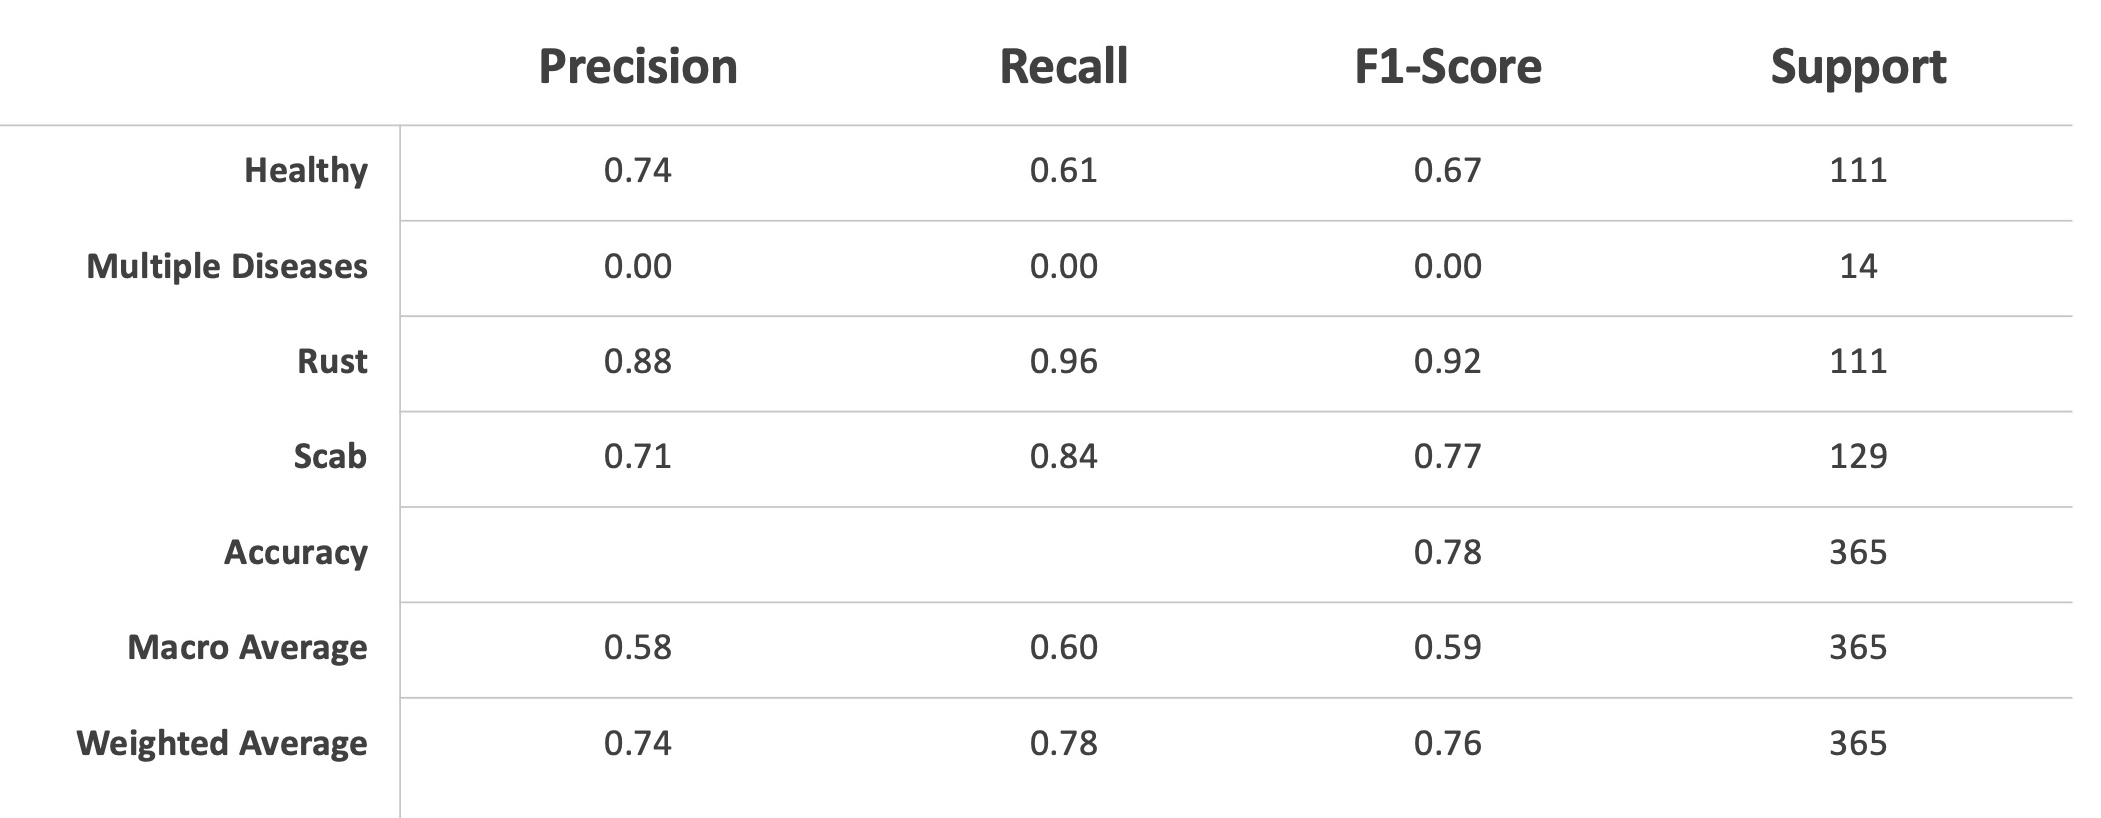
\includegraphics[width=1\textwidth]{images/image6.jpg}
%   \label{fig:Figure6}
% \end{figure}

\clearpage

\renewcommand{\arraystretch}{1.75}

\begin{table}[]
\centering
\caption{Classification Report}
\label{fig:Table1}
\begin{tabular}{|r|c|c|c|c|}
\hline
\multicolumn{1}{|l|}{}     & \multicolumn{1}{l|}{\textbf{Precision}} & \multicolumn{1}{l|}{\textbf{Recall}} & \multicolumn{1}{l|}{\textbf{F1-Score}} & \multicolumn{1}{l|}{\textbf{Support}} \\ \hline
\textbf{Healthy}           & 0.74                                    & 0.61                                 & 0.67                                   & 111                                   \\ \hline
\textbf{Multiple Diseases} & 0.00                                    & 0.00                                 & 0.00                                   & 14                                    \\ \hline
\textbf{Rust}              & 0.88                                    & 0.96                                 & 0.92                                   & 111                                   \\ \hline
\textbf{Scab}              & 0.71                                    & 0.84                                 & 0.77                                   & 129                                   \\ \hline
\textbf{Accuracy}          &                                         &                                      & 0.78                                   & 365                                   \\ \hline
\textbf{Macro Average}     & 0.58                                    & 0.60                                 & 0.59                                   & 365                                   \\ \hline
\textbf{Weighted Average}  & 0.74                                    & 0.78                                 & 0.76                                   & 365                                   \\ \hline
\end{tabular}
\end{table}

Overall, our model does a great job at detecting plants with rust, however, as I mentioned earlier in the report about plants with multiple diseases, our model clearly can’t find the pattern for this class label due to the lack of data on it.

To further improve the accuracy of the model, I decided to follow some of the steps that a 2016 research group did to obtain a 99.37$\%$ accuracy rate on a similar topic of image recognition of 26 plant diseases across 16 different plant species with over 55,000 samples in a controlled environment \parencite{frontiers}. They utilized transfer learning of pre-trained models such as GoogleNet and AlexNet to extend their version of CNN to classify the data. Pre-trained models like GoolgeNet and AlexNet have trained on over a million different images with 1000 class labels. What this means is that we can use the weights from these pre-trained models as a starting point for our model to hopefully improve accuracy. There are currently 18 pre-trained models on Keras API. So to see which model will be the most useful in helping us with our classification problem, we will calculate the performance of the pre-trained models by letting these models classify our data set. The weights of the model with the highest accuracy rate will be used as a starting point for the extended model.

After evaluating the 18 pre-trained models, Xception and DenseNet201 proved to be optimal for this problem. To utilize these models as feature extractors, we need to freeze all the layers when adding additional new layers to the model and then train it. The reason for this is because the new layers have randomized weights and therefore we don’t want it to update the weights of the base model (yet). After training, we can unfreeze all the base model’s layers and recompile our model so that the inner layers can take account to the new layer’s weights. Figure~\ref{fig:Figure6} shows the performance of the two models.
\clearpage

\begin{figure}
  \centering
  \caption{Base Model Comparison}
  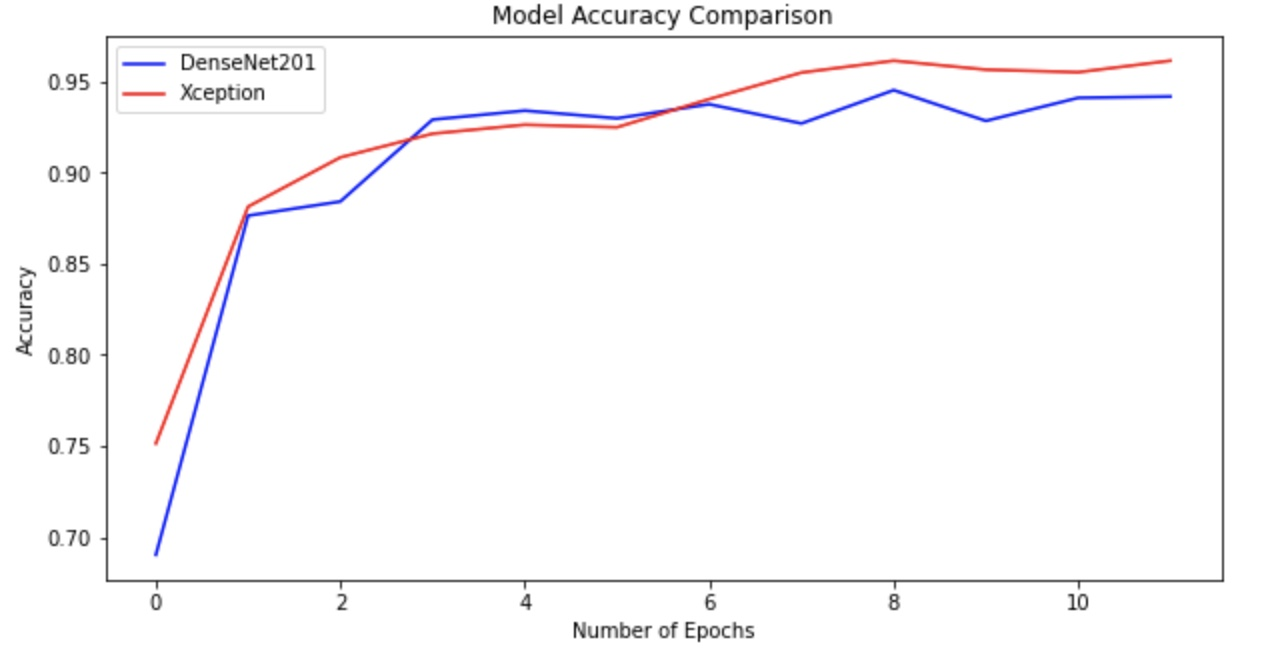
\includegraphics[width=0.8\textwidth]{images/image7.jpg}
  \label{fig:Figure6}
\end{figure}


As you can see, DenseNet201 and Xception obtain similar results of achieving over 93$\%$ accuracy. This is a 14$\%$ improvement from the original model which is a big leap in model
performance.


\section{Summary}
With the recent advances in image recognition and high-quality image capturing mobile devices, we can use different machine learning methods to help farmers detect various diseases
across different plant species. This is just the initial stage of the project. There are more steps that could have been taken to further improve the performance of these models. For example,
we could have generated more samples using Generative Adversarial Networks, create a segmentation model to remove the background noise and tune the parameters to achieve an even greater result.

After all, our sample size was relatively small, yet we were able to achieve a 94$\%$ accuracy after performing various steps such as data preprocessing where we resize, reshape and augment the images to provide more samples and better input for our model and achieving an 80$\%$ accuracy. Then we extended our model by embedding a pre-trained model on the top layer so that it can detect important features where we were able to achieve such high accuracy.


\section{Resources}
The data and code used in this project are available at the following location:

- Data: \url{https://www.kaggle.com/c/plant-pathology-2020-fgvc7/}

- Code: \url{https://github.com/bitngu/Image-Recognition-Plant-Pathology}

\printbibliography

\end{singlespace}
\end{document}

%% 
%% Copyright (C) 2019 by Daniel A. Weiss <daniel.weiss.led at gmail.com>
%% 
%% This work may be distributed and/or modified under the
%% conditions of the LaTeX Project Public License (LPPL), either
%% version 1.3c of this license or (at your option) any later
%% version.  The latest version of this license is in the file:
%% 
%% http://www.latex-project.org/lppl.txt
%% 
%% Users may freely modify these files without permission, as long as the
%% copyright line and this statement are maintained intact.
%% 
%% This work is not endorsed by, affiliated with, or probably even known
%% by, the American Psychological Association.
%% 
%% This work is "maintained" (as per LPPL maintenance status) by
%% Daniel A. Weiss.
%% 
%% This work consists of the file  apa7.dtx
%% and the derived files           apa7.ins,
%%                                 apa7.cls,
%%                                 apa7.pdf,
%%                                 README,
%%                                 APA7american.txt,
%%                                 APA7british.txt,
%%                                 APA7dutch.txt,
%%                                 APA7english.txt,
%%                                 APA7german.txt,
%%                                 APA7ngerman.txt,
%%                                 APA7greek.txt,
%%                                 APA7czech.txt,
%%                                 APA7turkish.txt,
%%                                 APA7endfloat.cfg,
%%                                 Figure1.pdf,
%%                                 shortsample.tex,
%%                                 longsample.tex, and
%%                                 bibliography.bib.
%% 
%%
%% End of file `./samples/longsample.tex'.
